\chapter{Diagrammi di Bode}
\section{Rappresentazione della funzione di trasferimento}

%TODO: Io la riscrivo, ma forse è meglio fare riferimento al capitolo 3 e magari metterci un link sul capitolo 3 e sottolineare la formula della funzione di trasferimento

%TODO: inserire una riga d'intestazione per non fare iniziare la sezione con una formula centrale

\begin{equation}
	H(j\omega) \dot{=}\int_{-\infty}^{+\infty} \! h(t)e^{-j\omega t} \d t
\end{equation}
dato uno specifico $\omega$ abbiamo un risultato nel piano complesso:
\[
	H(j\omega) \big\vert_{\omega = \omega_k}
\]

%TODO non so dove piazzare questo diagramma nel contesto
%TODO: fare immagine
\begin{figure}[H]
	\centering
	\includegraphics[width=0.7\linewidth]{immagini/cap6_Bode/diagNyquist}
	\caption{ Diagramma di nyquist: la funzione di trasferimento viene rappresentata come una curva parametrica al variare di $\omega$.  }
	\label{fig:diagNyquist}
\end{figure}

La rappresentazione su grafici rende più facile l'interpretazione della funzione di trasferimento. Per semplicità si può dividere il segnale nel modulo e nella fase.

\begin{equation*}
\begin{align}
 A(\omega)&=\abs{H(j\omega)}=\Abs{\int_{-\infty}^{+\infty} \! h(t)e^{-j\omega t} \d t} &\text{funzione pari}\\	
 \Phi (\omega)&= \arg(H(j\omega)) & \text{funzione dispari}
\end{align}
\end{equation*}

Rappresentiamo un numero complesso $z=a+jb$

\begin{equation*}
	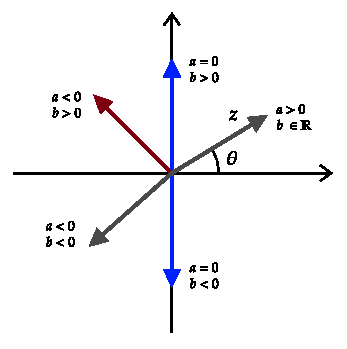
\includegraphics[width=0.3\linewidth]{immagini/cap6_Bode/argCompl}\quad
	\arg(z) =
	\begin{cases}
		\arctan \big(\frac{b}{a}\big) &,a>0, b\in \R\\
		\frac{\pi}{2}&,a=0, b>0\\
		-\frac{\pi}{2}&,a=0, b<0\\
		\arctan \big(\frac{b}{a}\big)+\pi &,a<0, b\ge 0\\
		\arctan \big(\frac{b}{a}\big)-\pi &,a<0, b< 0
	\end{cases}
\end{equation*}

Vista l'ampiezza delle possibili frequenze, usualmente si usa una scala logaritmica per esse. Vediamo come usare il logaritmo nei numeri complessi.

Nei reali: 
\begin{equation*}
	y=\ln (x) \iff x e^y, \quad x \in \R, y \in \R 
\end{equation*}
Nei complessi: %TODO da risistemare
\begin{gather*}
	w = \ln (z) \iff z=e^w \quad z \in \C^*, w \in \C \\
	z=\rho e^{j \theta} \quad w=u+jv\\
	z= \rho e^{j \theta} = e^w=e^{u+jv} = e^u e^{jv}\\
	\rho = e^u \rightarrow u = \ln(\rho) \rightarrow u =\ln(\abs{z})\\
	e^{j\theta} = e^{jv} \rightarrow v = \theta \rightarrow v= \arg (z)\\
	\ln (z) = w = u+jv = \ln (\abs{z}) + j \arg (z)
\end{gather*}

%TODO eh?
Logaritmo principale: dove $ -\pi < \arg (z) < \pi $ (oppure $ 0< \arg (x) <2\pi $)

\subsubsection{Proprietà del logaritmo}
\begin{enumerate}
	\item $ \ln ( b c) = \ln (b) + \ln (c) $
	\item $ \ln \Big(\frac{b}{c}\Big) = \ln (b) - \ln (c) $
	\item $ \ln (b^c) = c \ln (b) \quad ,c \in \R$
	\item $ \log_a (b)  = \frac{\log_c (b)}{\log_c (a)}=\frac{1)}{\log_c (a)}\log_c (b)$
\end{enumerate}

Per analogia:
\begin{enumerate}
	\item $ \arg ( b c) = \arg (b) + \arg (c) $
	\item $ \arg \Big(\frac{b}{c}\Big) = \arg (b) - \arg (c) $
	\item $ \arg (b^c) = c \arg (b) \quad ,c \in \R$
	\item Non c'è cambio di base
\end{enumerate}

\subsection{Decibel}
L'unità di misura dell'ampiezza nei diagrammi di Bode è il Decibel
\[
\abs{H(j\omega)}_{dB} = 20 \log_{10}\abs{H(j\omega)}
\]

%TODO nemmeno qui non so dove piazzare questo diagramma nel contesto
%TODO: fare immagine
\begin{figure}[H]
	\centering
	\includegraphics[width=0.7\linewidth]{immagini/cap6_Bode/diagNichols}
	\caption{ Rappresentazione logaritmica nel Diagramma di Nichols  }
	\label{fig:diagNichols}
\end{figure}

\section{Diagrammi di Bode}
%TODO: fare immagine
\begin{figure}[H]
	\centering
	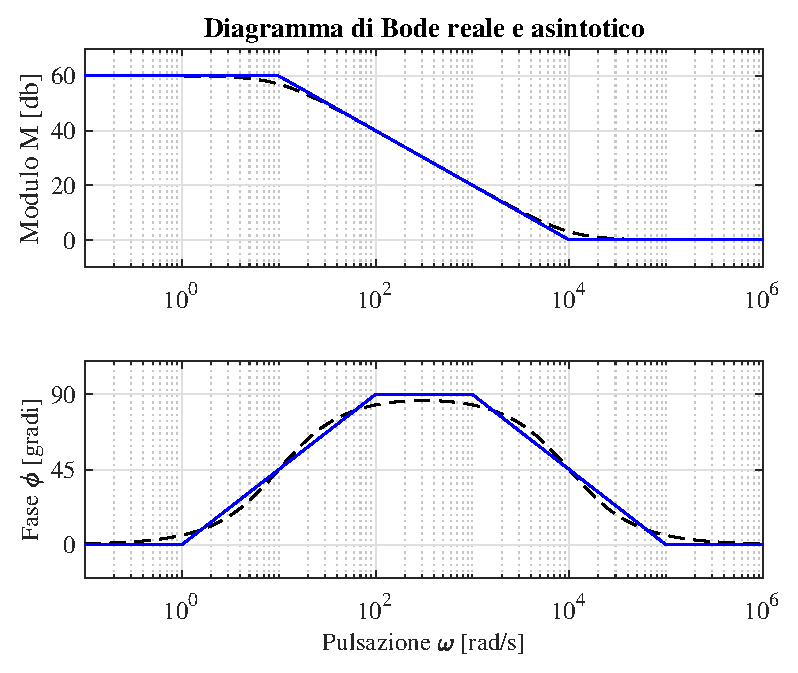
\includegraphics[width=0.7\linewidth]{immagini/cap6_Bode/diagBode}
	\label{fig:diagBode}
\end{figure}

%TODO introduzione migliore da fare

%TODO non so come introdurre i diseng sulle decadi
\begin{figure}[H]
	\centering
	\includegraphics[width=0.7\linewidth]{immagini/cap6_Bode/schDecade}
	\label{fig:schDecade}
\end{figure}
Considerando un punto nella decade tra $ 0 $ e $ 1 $ specifichaimo per gli esercizi
\[ 
	\log 2 \simeq 0,3 \quad \log 3 \simeq 0,5 \quad\log 5 \simeq 0,7 \quad\log 8 \simeq 0,9 
 \]
\begin{figure}[H]
	\centering
	\includegraphics[width=0.7\linewidth]{immagini/cap6_Bode/schDecade2}
	\label{fig:schDecade2}
\end{figure}

\[ 
	\ln (H(j\omega)) = \underbrace{\ln (A(\omega))}_{\text{daigramma Ampiezze}} + j\,\underbrace{\Phi (\omega)}_{\text{diagramma Fase}}
 \]
 
 In caso di un sistema:
 \begin{figure}[H]
 	\centering
 	\includegraphics[width=0.7\linewidth]{immagini/cap6_Bode/sist1}
 	\label{fig:sist1}
 \end{figure}

\[ 
	H(j \omega)=A(j \omega)B(j \omega)
 \]
 di conseguenza: 
 \[ 
	\ln H(j \omega)=\ln A(j \omega) + \ln B(j \omega)
 \]
 
 
 %TODO Questo cos'é? Un altra section? Non so che titolo mettere
 
 Possiamo scrivere $ H(s) $ come:
 \[  
 	K \, \frac{(s-z_1)\,(s-z_2)\,\dots \,(s-z_m)}{(p-z_1)\,(p-z_2)\,\dots \,(p-z_m)}
 \]
 in forma \emph{irriducibile} con $K \in \R  $, $ z_i $ zeri di $ H(s) $ e $ p_i $ poli di $ H(s) $
 
 Possiamo avere tre casi:
 \begin{enumerate}
 	\item $ z_1=0 $ e/o $ p_i = 0 $ cioè poli nell' \\
 	\item $ (s-z_i) $ e/o $ (s-p_i) $ non nulli ($ \ne 0  \wedge \in \R$)\\
 	\item poli complessi coniugati: $ (s-z_i)(s-\overline{z_i}) $ e/o  $ (s-p_i)(s-\overline{p_i}) $
 \end{enumerate}

\subsubsection{Caso 1}
Avremo un termine di questo tipo al denominatore:
 $ \frac{1}{s^\nu}  $
con 
\begin{itemize}
	\item $ \nu =0 $ Se $ H(s) $ non ha poli o zeri nell'origine\\
	\item $ \nu >0 $ Se $ H(s) $ ha polo nell'origine di molteplicità $ \nu $\\
	\item $ \nu <0 $ Se $ H(s) $ ha zeri nell'origine di molteplicità $\nu$
\end{itemize}

\subsubsection{Caso 2}
Zeri: $ s-z_i \quad z_i \ne 0 $
\[ 
	(s-z_i)=(-z_i)\Big(1+s \frac{1}{-z_1} \Big)=(-z_i)(1+s \tau'_i) \qquad \tau'_i \dot{=} \frac{1}{-z_i}
 \]
 
 (In questo caso $ \tau'_i $ non ha seignificato fisico) %TODO ho capito bene?
 
 Equivalentemente per i poli: $ s-p_i \quad p_i \ne 0 $
 \[ 
 (s-p_i)=(-z_i)\Big(1+s \frac{1}{-p_1} \Big)=(-p_i)(1+s \tau_i) \qquad \tau_i \dot{=} \frac{1}{-p_i} \, \text{Costante di tempo}
 \]
 %TODO nei miei appunti è l al posto di e e nell'ultima parte p al posto di Tau, purtroppo non ho trovato sul libro un riferimento 
 \[ (s-p_i) \rightarrow e^{p_i t} \rightarrow e^{-\frac{t}{\tau_1}} \, \text{decadimento esponenziale}\]
 
 \subsubsection{Caso 3}
 \[ 
 	(s-z_k)(s-\overline{z_k}) = s^2-z_ks-\overline{z_k}s+z_k \,\overline{z_k} = \Re(z_k) s+\abs{z_k}^2 = \abs{z_k}^2\Big(1-\frac{2 \Re(z_k)}{\abs{z_k}}\frac{s}{\abs{z_k}}+\frac{s^2}{\abs{z_k}} \Big)
 \]

 Definiamo $ \omega'_n \dot{=} \abs{z_k} $ come \emph{pulsazione naturale} e $ \zeta_k \dot{=} \frac{-\Re(z_k)}{\abs{z_k}} $ come \emph{fattore di smorzamento}, di conseguenza abbiamo: 
 \[ 
 	(s-z_k)(s-\overline{z_k}) = \abs{z_k}^2\Big(1+2\zeta'_k\frac{s}{\omega'_{nk}}+\frac{s^2}{\omega^{'2}_{nk}} \Big)
  \]
  
  Analogalmente con $ \omega_n \dot{=} \abs{p_k} $ e $ \zeta_k \dot{=} \frac{-\Re(p_k)}{\abs{p_k}} $ abbiamo:
   \[ 
  (s-p_k)(s-\overline{p_k}) = \abs{p_k}^2\Big(1+2\zeta_k\frac{s}{\omega_{nk}}+\frac{s^2}{\omega^{2}_{nk}} \Big)
  \]
  
  Ora possiamo riscrivere la funzione di trasferimento in $ s $:
  \[ 
  	H(s) = K_B \, \frac{\prod_i (1+s\tau'_i)^{\mu'_i}\,  \prod_k \Big(1+2\zeta'_k\frac{s}{\omega'_{nk}}+\frac{s^2}{\omega^{'2}_{nk}} \Big)^{\mu'_k}}{s^\nu\, \prod_i (1+s\tau_i)^{\mu_i}\,  \prod_k \Big(1+2\zeta_k\frac{s}{\omega_{nk}}+\frac{s^2}{\omega^{2}_{nk}} \Big)^{\mu_k} }
   \]